\documentclass[10pt]{article}

% Manuscript v5 (draft, 18 Nov 2026): empirical AI-architecture framing.
% Same evidence as v4; formal results moved to Appendix A except the repair-acceptance
% theorem, which the experiments test directly. Every number comes from a saved run
% (Appendix F). \pending{...} marks results of the running factorial study.
\usepackage[letterpaper,margin=1in]{geometry}
\usepackage{times}
\usepackage{amsmath,amssymb,amsthm}
\usepackage{booktabs}
\usepackage{graphicx}
\usepackage{array}
\usepackage{multirow}
\usepackage{xcolor}
\usepackage{float}
\usepackage{algpseudocode}
\usepackage[round]{natbib}
\usepackage{hyperref}
\hypersetup{colorlinks=true,linkcolor=blue,citecolor=blue,urlcolor=blue}
\emergencystretch=2em

\newfloat{algorithm}{tbp}{loa}
\floatname{algorithm}{Algorithm}
\theoremstyle{plain}
\newtheorem{proposition}{Proposition}
\newtheorem{lemma}{Lemma}
\newtheorem{theorem}{Theorem}
\newtheorem{corollary}{Corollary}
\theoremstyle{definition}
\newtheorem{assumption}{Assumption}

\newcommand{\asem}{\textsc{ASEM}}
\newcommand{\care}{\textsc{CARE}}
\newcommand{\pending}[1]{\textcolor{red}{\textbf{[PENDING: #1]}}}
\newcommand{\sub}{\sqsubseteq}
\newcommand{\A}{\mathcal{A}}
\newcommand{\D}{\mathcal{D}}
\newcommand{\G}{\mathcal{G}}
\newcommand{\F}{\mathcal{F}}

\title{\textbf{Source-Anchored Graph Memory with Bounded Repair\\
for Long-Horizon Conversational Question Answering}}
\author{Anonymous authors\\ \small Draft v5 --- not under review}
\date{}

\begin{document}
\maketitle

\begin{abstract}
Conversational agents must answer questions about histories far longer than their context
window. We present \asem{}, a memory architecture that keeps every original turn in an
append-only archive as the only citable evidence, builds a four-layer memory graph over it
(turns, entities, sessions, communities) without an LLM, and answers with a bounded reader that
cites source turns and may repair its answer once, using lexical, dense or graph-PPR expansion.
A guarded write path stores versioned notes whose values must be quoted from a turn. We evaluate
with open models only (Qwen3-8B reader, Qwen3-Embedding-0.6B encoder) on all 1,986 LoCoMo questions
and all 500 LongMemEval cleaned-oracle questions. With the same reader, \asem{}'s repair raises the
LoCoMo score from 0.459 to 0.526, far above full-context (0.196) and dense-RAG (0.407) baselines, but
reverses 46 correct refusals; a dense first bundle beats BM25 before repair ($+0.014$, 9 of 10
conversations) and matches it after repair. We show that a repair verifier must catch refusal-losing
repairs 3.89 times as often as it rejects useful ones, and that all six verifiers we built fall below
this bound, as predicted. A pre-registered $2\times3$ factorial over first bundle and repair type,
including the graph arm, is reported in Section~\ref{sec:ablation}: \pending{headline of the factorial
study}.
\end{abstract}

% =====================================================================================
\section{Introduction}
\label{sec:intro}

Long-running agents answer questions whose evidence was said months earlier, has since been
updated, or belongs to a different speaker. Two families of memory systems address this. Write-time
systems extract, link and consolidate memories as the conversation arrives
\citep{packer2023memgpt,chhikara2025mem0,amem2025,memoryr12025,cao2026higmem}; read-time systems keep
the history and decide per question what to read \citep{du2026memr3,wang2026cuemem,liu2026livectx,chen2026justmem,yu2026lazymem}.
Corrective retrieval-augmented generation sits between them, retrieving again when a first answer
looks unsupported \citep{jiang2023active,asai2023selfrag,yan2024crag}.

We design \asem{} around three empirical observations from our own failure analysis. First, an answer
is only as trustworthy as its link to an original turn, so the original turns must never be rewritten.
Second, a small reader often has the evidence and still answers wrongly, so read-time retrieval alone
has a ceiling. Third, a second read helps answerable questions but can talk the reader out of a
correct refusal, so the repair step must be bounded and its acceptance understood.

\begin{figure}[t]
\centering
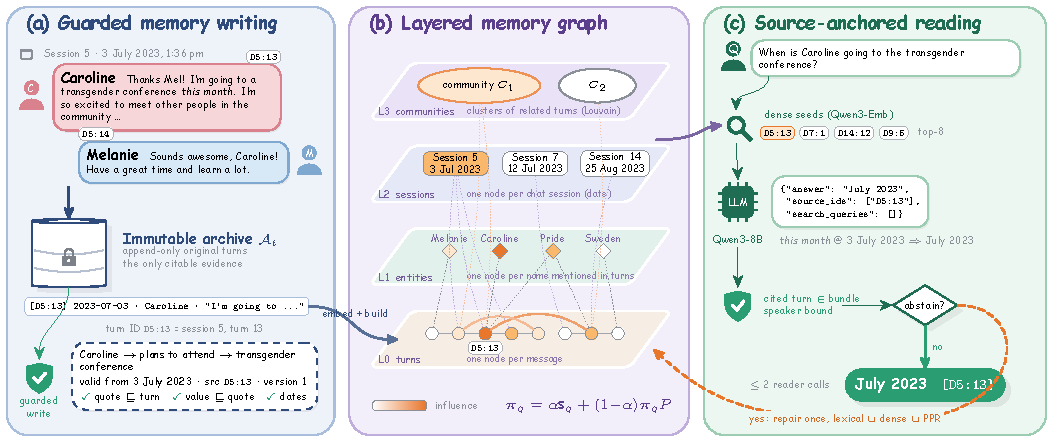
\includegraphics[width=\linewidth]{figures/asem_method_figure.pdf}
\caption{\asem{} overview. \textbf{(a)} Original turns enter an append-only archive, the only citable
evidence; guarded operators write versioned notes whose values must be quoted from a turn (dashed:
implemented and unit-tested, not yet evaluated end to end). \textbf{(b)} A four-layer memory graph is
built per conversation without an LLM; a question's personalized-PageRank mass gives each node its
influence. \textbf{(c)} The reader answers from a top-8 first bundle with cited source IDs, code checks
bind the citations to the bundle, and an abstention with missing-evidence searches triggers at most one
graph-aware repair. The example is real (LoCoMo \texttt{conv-26}, question 17): the turns, the dense
top-4 seeds and the answer \emph{July 2023} citing \texttt{D5:13} are saved outputs of our run. Node
shading and community memberships in (b) illustrate the mechanism.}
\label{fig:overview}
\end{figure}

\paragraph{Contributions.}
\begin{enumerate}
  \item \textbf{Architecture.} A source-anchored memory with an immutable archive, a layered memory
  graph with personalized-PageRank influence, a citation-checked bounded reader, and three repair
  expansions (lexical, dense, graph) behind one gate (Section~\ref{sec:method}).
  \item \textbf{A controlled empirical study with open models.} Nine systems on the same 1,986 LoCoMo
  questions with one reader; 500 LongMemEval questions; a pre-registered factorial ablation with
  development/test separation; exact reproducibility checks (Sections~\ref{sec:setup}--\ref{sec:results}).
  \item \textbf{An account of the repair trade-off.} Repair consistently converts correct refusals into
  answers; we derive the condition under which any verifier can recover them and confirm it on six
  verifiers (Sections~\ref{sec:accept} and~\ref{sec:abstention}).
  \item \textbf{Findings that change design choices.} A current open encoder reverses an earlier
  sparse-over-dense conclusion; the retriever and repair step interact; graph influence helps at repair
  budgets, not first-bundle budgets; the residual error is aggregation, not access
  (Sections~\ref{sec:retrieval} and~\ref{sec:errors}).
\end{enumerate}

% =====================================================================================
\section{Related Work}
\label{sec:related}

\paragraph{Persistent memory.} MemGPT pages information between context and storage
\citep{packer2023memgpt}; Mem0 extracts and consolidates facts \citep{chhikara2025mem0}; A-Mem links
and revises notes \citep{amem2025}; Memory-R1 learns write operations \citep{memoryr12025}; HiGMem keeps
an event--turn hierarchy whose summaries are refreshed online \citep{cao2026higmem}. Their updates are
prompted or learned; \asem{} adds code-checked guards and keeps an immutable citation layer.

\paragraph{Read-time access.} MemR$^3$ tracks evidence gaps while routing among retrieval and answering
\citep{du2026memr3}; CueMem and LiveCtx rebuild context from raw turns \citep{wang2026cuemem,liu2026livectx};
JustMem selects lookup, composition or source replay per query over atomic cards
\citep{chen2026justmem}; LazyMem builds a compact memory at query time with a 4B keep/drop model
\citep{yu2026lazymem}.

\paragraph{Graph and corrective retrieval.} Personalized PageRank gives seed-centred, local relevance
\citep{andersen2006local}; HippoRAG applies it to long-term memory \citep{gutierrez2024hipporag}.
FLARE, Self-RAG, Adaptive-RAG and CRAG decide when to retrieve again or how to correct evidence
\citep{jiang2023active,asai2023selfrag,jeong2024adaptive,yan2024crag}; our acceptance analysis concerns
the decision they share: whether to keep the second answer.

% =====================================================================================
\section{Method}
\label{sec:method}

\subsection{Memory representation}

A conversation is a stream of turns $s_i=(\mathrm{id}_i,\sigma_i,t_i,p_i,x_i)$ with session $\sigma_i$,
session date $t_i$, speaker $p_i$ and text $x_i$. \asem{} keeps
\begin{equation}
M_t=(\A_t,\ \D_t,\ \G_t),\qquad \A_t=\{s_i:i\le t\},
\label{eq:state}
\end{equation}
an append-only \emph{archive} $\A_t$ (the only source a final answer may cite), a \emph{derived layer}
$\D_t$ of versioned notes, and a \emph{memory graph} $\G_t$ built over both. A note
$n=(k,v,\mathrm{Src},\tau,\mathrm{ver},\mathrm{st})$ stores a value $v$ for a key
$k=(\text{subject},\text{attribute})$, its source turns, its validity date, a version and a status.

\subsection{Layered memory graph}
\label{sec:graph}

For each history, $\G_t$ has four node layers: turns $V_0=\A_t$, entities $V_1$, sessions $V_2$ and
communities $V_3$. Turn $i$ carries an embedding $e_i$ from the encoder. Edges and weights are
\begin{equation}
w_{ij}=\begin{cases}
1 & j=i+1,\ \sigma_j=\sigma_i \quad(\textsf{next})\\
\max(\cos(e_i,e_j),0) & j\in\mathrm{NN}_5(i)\quad(\textsf{semantic})\\
0.5 & i\in V_0,\ j\in V_1,\ \text{$x_i$ mentions $j$}\\
0.3 & i\in V_0,\ j\in V_2\cup V_3,\ \text{$i$ belongs to $j$},
\end{cases}
\label{eq:edges}
\end{equation}
where entities are capitalized tokens occurring in at least 2 and at most $5\%$ of the turns, and
communities are Louvain clusters (fixed seed) of the turn subgraph. No LLM is called to build $\G_t$.

\subsection{Retrieval: hybrid seeds and graph influence}

Turns are scored lexically by BM25 ($k_1{=}1.5$, $b{=}0.75$) and densely by
$\mathrm{sim}(q,i)=\langle e_Q(q),e_i\rangle$ with an instruction-prefixed query embedding. Rankings can be
fused by reciprocal rank \citep{cormack2009rrf},
\begin{equation}
\mathrm{rrf}(i)=\sum_{j\in\{\mathrm{bm25},\mathrm{dense}\}}\big(60+\rho_j(i)\big)^{-1}.
\label{eq:rrf}
\end{equation}
For graph retrieval, a uniform restart distribution $\mathbf{s}_q$ over the five best dense turns seeds a
personalized PageRank on the row-normalized transition matrix $P$ of~\eqref{eq:edges},
\begin{equation}
\boldsymbol\pi_q=\alpha\,\mathbf{s}_q+(1-\alpha)\,\boldsymbol\pi_q P,\qquad \alpha=0.5,
\label{eq:ppr}
\end{equation}
and a turn's \emph{influence} $\pi_q(i)$ is combined with its dense score,
\begin{equation}
r_q(i)=\lambda\, z\big(\mathrm{sim}(q,i)\big)+(1-\lambda)\,z\big(\pi_q(i)\big),\qquad \lambda=0.7,
\label{eq:mix}
\end{equation}
with $z$ the z-score over the history's turns. $\lambda$ was selected on development data
(Section~\ref{sec:retrieval}). Lemma~\ref{lem:ppr} (Appendix~\ref{app:proofs}) bounds the influence that
leaks beyond $h$ hops of the seeds by $(1-\alpha)^{h+1}$.

\subsection{Source-anchored reader and repair gate}

The first bundle $B_1$ is the top eight turns under BM25 or dense scoring, serialized with ID, date and
speaker under $L=10{,}000$ characters. The frozen reader returns
\begin{equation}
(a,\,C,\,Q)=R_\theta(q,B),\qquad C\leftarrow C\cap\mathrm{ids}(B),\qquad a\leftarrow\bot\ \text{if } C=\varnothing,
\label{eq:reader}
\end{equation}
an answer, cited source IDs filtered to the visible bundle, and at most two searches $Q$ for missing
evidence. A speaker-binding and two event checks can invalidate a pass ($r=1$). Repair fires when
\begin{equation}
\tau(q)=\mathbf{1}\big[r_1\ \lor\ \big(a_1=\bot\ \land\ (Q_1\neq\varnothing\ \lor\ \rho(q))\big)\big],
\label{eq:gate}
\end{equation}
where $\rho$ flags temporal, update or aggregation cues.

\subsection{Bounded repair with three expansions}
\label{sec:repair}

When $\tau(q)=1$, the reader is called once more on an expanded bundle $B_2$. Let $E_{\mathrm{lex}}$ be the
lexical expansion of \care{}: the top-18 unstemmed and stemmed BM25 turns, session neighbours of the
leading hits, and six unstemmed and six stemmed hits for each search in $Q_1$. With $D_k(x)$ and
$G_k(x)$ the top-$k$ turns of text $x$ under dense similarity and under~\eqref{eq:mix},
\begin{align}
E_{\mathrm{hyb}}&=E_{\mathrm{lex}}\ \cup\ D_6(q)\ \cup\ \textstyle\bigcup_{s\in Q_1}D_6(s), \label{eq:hyb}\\
E_{\mathrm{graph}}&=E_{\mathrm{lex}}\ \cup\ G_6(q)\ \cup\ \textstyle\bigcup_{s\in Q_1}G_6(s). \label{eq:graphrep}
\end{align}
The expanded pool is restored to conversation order and cut at $L$ characters. Every question therefore
costs $1+\tau(q)\le2$ reader calls.

\subsection{Guarded write path}

Notes are written only through operators whose guards are checked in code: \textsc{Add} requires a
quote $w$ with $w\sub x_s$ for a cited archive turn $s$ and $v\sub w$; \textsc{Update} additionally
requires the new evidence not to predate the current version (dates are parsed, not compared as strings)
and keeps the old version as \emph{superseded}; \textsc{Link} admits only typed edges between notes that
share a session or a turn. Rejected writes are logged. The write path is implemented and unit-tested but
not yet part of the evaluated pipeline.

\paragraph{Properties.} Under an append-only archive and exact guards, every stored note is grounded in
an archive turn, each key has at most one current version with ordered validity dates, the derived layer
can be rebuilt from the log, every reader bundle consists of archive turns, and count errors of an
aggregation over notes decompose into missed, duplicated and misinterpreted notes
(Propositions~\ref{prop:grounding}--\ref{prop:agg}, Appendix~\ref{app:proofs}). These guarantee
traceability and bounded cost, not correctness.

\subsection{When should a repair be accepted?}
\label{sec:accept}

A \emph{flip} is a repair that turns a first-pass abstention into an answer. Let $\F^+$ and $\F^-$ be flips
on answerable and unsupported questions. Accepting flip $f$ changes the total score by
$d_f=m(a_2,y)-m(\bot,y)$, which lies in $[0,1]$ on $\F^+$ and equals $-1$ on $\F^-$. Let
$G=\sum_{\F^+}d_f$ and $L=|\F^-|$. A verifier $V:\F\to\{0,1\}$ keeps flip $f$ iff $V(f)=1$.

\begin{theorem}[Break-even]
\label{thm:breakeven}
$\Delta_V-\Delta_{\mathrm{all}}=L^{\mathrm{caught}}_V-G^{\mathrm{rej}}_V$, where $L^{\mathrm{caught}}_V$ counts
rejected flips in $\F^-$ and $G^{\mathrm{rej}}_V$ sums $d_f$ over rejected flips in $\F^+$.
\end{theorem}
\begin{proof}
$\Delta_{\mathrm{all}}-\Delta_V=\sum_{V(f)=0}d_f=G^{\mathrm{rej}}_V-L^{\mathrm{caught}}_V$.
\end{proof}

\begin{corollary}[Rate condition]
\label{cor:rate}
If $V$ rejects flips in $\F^-$ with probability $\alpha$ and flips in $\F^+$ with probability $\beta$,
independently of $d_f$, then $\mathbb{E}[\Delta_V-\Delta_{\mathrm{all}}]=\alpha L-\beta G$; $V$ helps iff
$\alpha/\beta>G/L$.
\end{corollary}

The threshold $G/L$ depends only on the data and the reader. Section~\ref{sec:abstention} measures it and
tests the prediction.

% =====================================================================================
\section{Experimental Setup}
\label{sec:setup}

\paragraph{Benchmarks and protocol.} \emph{LoCoMo} \citep{maharana2024locomo}: ten conversations, 5,882
turns, 1,986 questions in five categories (multi-hop 282, temporal 321, open-domain 96, single-hop 841,
adversarial 446, following the A-Mem and HiGMem naming \citep{amem2025,cao2026higmem}). LoCoMo was used
during development and serves as the \textbf{development} set. \emph{LongMemEval} cleaned oracle
\citep{wu2024longmemeval}: 500 questions over the annotated sessions (948 sessions, 10,960 turns), 30 of
them abstention questions; it is the \textbf{test} set and is run once with frozen code. Arms, metrics,
hypotheses and the code hash were registered before the factorial run (Appendix~\ref{app:protocol}).

\paragraph{Systems.} Table~\ref{tab:systems} lists every system. All share the reader, decoding and
evidence budget; ``-8'' systems also share \asem{}'s prompt, citation checks and gate.

\begin{table}[t]
\centering
\caption{Systems in the study. The factorial crosses the first bundle with the repair expansion; all
\asem{} variants use the same reader, prompt, checks and gate.}
\label{tab:systems}
\small
\begin{tabular}{llll}
\toprule
Group & System & First bundle & Repair \\
\midrule
\multirow{3}{*}{Baselines} & NoMemory & none & -- \\
 & FullContext-8K & first 5 turns + longest recent suffix in 8K & -- \\
 & Dense RAG (MiniLM, Qwen3-Emb) & dense top-18, plain RAG prompt & -- \\
\midrule
\multirow{7}{*}{\asem{} factorial} & BM25-8 / first pass & BM25 top-8 & none \\
 & BM25-8 / lexical (= \care{}) & BM25 top-8 & $E_{\mathrm{lex}}$ \\
 & BM25-8 / hybrid & BM25 top-8 & $E_{\mathrm{hyb}}$ \\
 & Dense-8 / first pass & dense top-8 & none \\
 & Dense-8 / lexical & dense top-8 & $E_{\mathrm{lex}}$ \\
 & Dense-8 / hybrid (\textbf{proposed}) & dense top-8 & $E_{\mathrm{hyb}}$ \\
 & Dense-8 / graph & dense top-8 & $E_{\mathrm{graph}}$ \\
\bottomrule
\end{tabular}
\end{table}

\paragraph{Metrics and statistics.} LoCoMo uses the benchmark scorer (per-item F1 for multi-hop,
stemmed-token F1 for other answerable categories, refusal phrase match for adversarial); the aggregate is
the mean per-question score. LongMemEval uses a diagnostic token F1 on answerable questions and
phrase-based abstention; it is not the official judged accuracy, so published LongMemEval numbers are not
comparable. We also report correct refusals, answerable questions answered with $\bot$, reader calls and
server-counted tokens. LoCoMo intervals resample the ten conversations (10,000 draws) and we report how
many conversations favour each system; LongMemEval intervals resample questions. The four primary
hypotheses use Bonferroni-adjusted 98.75\% intervals.

\paragraph{Implementation.} Table~\ref{tab:impl} lists the configuration. All models are open-weights.

\begin{table}[t]
\centering
\caption{Implementation details (fixed for all runs).}
\label{tab:impl}
\small
\begin{tabular}{l>{\raggedright\arraybackslash}p{13.4cm}}
\toprule
Reader & Qwen3-8B \citep{yang2025qwen3}, pinned revision, fp16, vLLM, non-thinking, temperature 0, $\le$224 output tokens \\
Encoder & Qwen3-Embedding-0.6B \citep{zhang2025qwen3embedding}, pinned, fp16, last-token pooling, docs $\le$1,024 tokens \\
Hardware & Kaggle, 2$\times$NVIDIA T4 (tensor parallel 2), 8,192-token window, one sequence at a time \\
Evidence & first bundle 8 turns; $L=10{,}000$ characters per call; repair $\le 1$; $k_{\mathrm{RRF}}=60$ \\
Graph & 5-NN semantic edges; entity df in $[2,\,5\%]$; Louvain seed 20261117; PPR $\alpha=0.5$, 5 seeds, 40 iterations; $\lambda=0.7$ \\
Repair & $E_{\mathrm{lex}}$ as in \care{}; dense or graph additions $k=6$ per query \\
\bottomrule
\end{tabular}
\end{table}

% =====================================================================================
\section{Results}
\label{sec:results}

\subsection{Main comparison on LoCoMo}
\label{sec:main}

\begin{table}[t]
\centering
\caption{All systems on the same 1,986 LoCoMo questions with the same Qwen3-8B reader. ``Refused ans.''
counts answerable questions answered with $\bot$ (of 1,540). Tokens are server-counted input plus output
per question.}
\label{tab:main}
\small
\begin{tabular}{lrrrrrr}
\toprule
System & Score & Answerable & Correct refusals & Refused ans. & Calls & Tokens/q \\
\midrule
NoMemory & 0.0774 & 0.0998 & 0/446 & 2 & 1,986 & 78 \\
FullContext-8K & 0.1961 & 0.2406 & 19/446 & 40 & 1,986 & 7,888 \\
Dense RAG (MiniLM, top-18) & 0.4069 & 0.3124 & 327/446 & 387 & 1,986 & 1,124 \\
\midrule
MiniLM-8 / first pass & 0.4168 & 0.2908 & 380/446 & 691 & 1,986 & 715 \\
BM25-8 / first pass & 0.4588 & 0.3489 & 374/446 & 630 & 1,986 & 715 \\
Dense-8 / first pass & \textbf{0.4730} & \textbf{0.3775} & 358/446 & 469 & 1,986 & 751 \\
\midrule
MiniLM-8 / lexical repair & 0.4994 & 0.4415 & 312/446 & 245 & 3,056 & 1,920 \\
BM25-8 / lexical repair (\care{}) & \textbf{0.5256} & \textbf{0.4648} & \textbf{328/446} & 257 & 2,990 & 1,836 \\
Dense-8 / lexical repair & 0.5169 & 0.4640 & 312/446 & \textbf{219} & \textbf{2,813} & \textbf{1,678} \\
\bottomrule
\end{tabular}
\end{table}

Table~\ref{tab:main} compares systems that differ only in how they select and repair evidence. Every
\asem{} configuration beats the context baselines by a wide margin: FullContext-8K keeps only 25.8\% of
the turns of each history, and dense RAG with a plain prompt reaches 0.4069. Among first passes, the
Qwen3-Embedding bundle beats BM25 by $+0.0142$ (conversation-cluster interval $[+0.0062,+0.0228]$, 9 of
10 conversations) and MiniLM by $+0.0562$ ($[+0.0405,+0.0728]$, 10 of 10). After lexical repair it
beats the MiniLM system by $+0.0175$ ($[+0.0088,+0.0266]$, 9 of 10) but not \care{}: $-0.0087$
($[-0.0183,+0.0013]$, 3 of 10). Answerable F1 is the same to three decimals (0.4640 versus 0.4648); the
difference is 16 refusals, worth 0.0081. The dense system is the cheapest repair system and refuses the
fewest answerable questions. Repair adds $+0.0667$ on top of BM25 and $+0.0826$ on top of MiniLM but
only $+0.0439$ on top of the dense bundle, so the first-bundle choice and the repair expansion interact;
the factorial study tests whether dense or graph additions to the repair restore the gain.

\subsection{Factorial ablation and the test set}
\label{sec:ablation}

\begin{table}[t]
\centering
\caption{Pre-registered factorial ablation. LoCoMo is development, LongMemEval (cleaned oracle) is test.
Scores are the primary metric of each benchmark.}
\label{tab:ablation}
\small
\begin{tabular}{lccccc}
\toprule
 & \multicolumn{2}{c}{LoCoMo (dev)} & \multicolumn{3}{c}{LongMemEval (test)} \\
\cmidrule(lr){2-3}\cmidrule(lr){4-6}
System & Score & Calls & Score & Correct abst. & Calls \\
\midrule
NoMemory & 0.0774 & 1,986 & \multicolumn{3}{c}{\pending{factorial}} \\
FullContext-8K & 0.1961 & 1,986 & \multicolumn{3}{c}{\pending{factorial}} \\
Dense RAG (Qwen3-Emb, top-18) & \multicolumn{2}{c}{\pending{factorial}} & \multicolumn{3}{c}{\pending{factorial}} \\
BM25-8 / first pass & \multicolumn{2}{c}{\pending{factorial}} & \multicolumn{3}{c}{\pending{factorial}} \\
BM25-8 / lexical (\care{}) & \multicolumn{2}{c}{\pending{factorial}} & \multicolumn{3}{c}{\pending{factorial}} \\
BM25-8 / hybrid & \multicolumn{2}{c}{\pending{factorial}} & \multicolumn{3}{c}{\pending{factorial}} \\
Dense-8 / first pass & \multicolumn{2}{c}{\pending{factorial}} & \multicolumn{3}{c}{\pending{factorial}} \\
Dense-8 / lexical & \multicolumn{2}{c}{\pending{factorial}} & \multicolumn{3}{c}{\pending{factorial}} \\
Dense-8 / hybrid (proposed) & \multicolumn{2}{c}{\pending{factorial}} & \multicolumn{3}{c}{\pending{factorial}} \\
Dense-8 / graph & \multicolumn{2}{c}{\pending{factorial}} & \multicolumn{3}{c}{\pending{factorial}} \\
\bottomrule
\end{tabular}
\end{table}

The pre-registered hypotheses are \textbf{H1} Dense-8/hybrid $>$ \care{}; \textbf{H2} Dense-8/hybrid $>$
Dense-8/lexical; \textbf{H3} Dense-8 first pass $>$ BM25-8 first pass; \textbf{H4} Dense-8/graph $>$
Dense-8/hybrid. Results: \pending{H1--H4 with 95\% and 98.75\% intervals}. The factorial reruns the
\care{} arm in the new harness; its answers are identical to the saved \care{} runs on every question
checked so far (673 of 673 across four shards), and the GPU-computed dense top-8 matches the frozen
rankings on 99.7\% of entries.

\subsection{Retrieval: encoder and graph}
\label{sec:retrieval}

\begin{table}[t]
\centering
\caption{Recall of annotated evidence in the top-$k$ ranking (no reader). Left: encoders on both
benchmarks. Right: layered-graph rankings on LoCoMo development data.}
\label{tab:retrieval}
\small
\begin{tabular}{lcccc@{\hspace{14pt}}lcc}
\toprule
 & \multicolumn{2}{c}{LoCoMo} & \multicolumn{2}{c}{LongMemEval} & Graph ranking (LoCoMo) & $k{=}8$ & $k{=}18$ \\
\cmidrule(lr){2-3}\cmidrule(lr){4-5}\cmidrule(lr){7-8}
Ranker & $k{=}8$ & $k{=}18$ & $k{=}8$ & $k{=}18$ & & & \\
\midrule
BM25 & 0.539 & 0.624 & 0.837 & 0.941 & dense only & 0.617 & 0.725 \\
BM25 (stemmed) & 0.578 & -- & 0.846 & -- & PPR only & 0.605 & 0.695 \\
Dense (Qwen3-Emb) & \textbf{0.617} & \textbf{0.725} & \textbf{0.926} & \textbf{0.988} & mix $\lambda{=}0.5$ & 0.617 & 0.735 \\
Hybrid RRF & 0.612 & -- & 0.911 & -- & mix $\lambda{=}0.7$ & \textbf{0.618} & \textbf{0.736} \\
 & & & & & community round-robin & 0.415 & -- \\
\bottomrule
\end{tabular}
\end{table}

An earlier comparison with MiniLM-L6-v2 had found BM25 ahead of dense retrieval (source recall 0.5353
versus 0.4576 at eight turns). With Qwen3-Embedding-0.6B the order reverses on both benchmarks
(Table~\ref{tab:retrieval}, left), in all ten LoCoMo conversations, with the largest gains where several
pieces of evidence are needed (LoCoMo multi-hop 0.225 to 0.378; LongMemEval multi-session 0.670 to
0.858). Fusion does not beat dense alone. The layered graph (on average 588 turns, 93 entities, 27
sessions and 10 communities per LoCoMo history) adds almost nothing at the first-bundle budget
($+0.001$) but $+0.011$ at a repair-sized budget of 18 turns (Table~\ref{tab:retrieval}, right); PPR alone
is worse than dense, and picking turns community by community hurts. We therefore use graph influence
only in the repair expansion~\eqref{eq:graphrep}, with $\lambda=0.7$ chosen on these development numbers.

\subsection{The abstention trade-off and repair acceptance}
\label{sec:abstention}

\begin{table}[t]
\centering
\caption{First pass versus lexical repair (\care{}), same reader. Left: both benchmarks. Right: acceptance
verifiers on the 419 LoCoMo flips; $\alpha$ is the share of unsupported flips rejected, $\beta$ the share
of answerable flips rejected; Corollary~\ref{cor:rate} requires $\alpha/\beta>3.89$.}
\label{tab:abstention}
\small
\begin{tabular}{llrr@{\hspace{14pt}}lrrr}
\toprule
Benchmark & Policy & Score & Refusals & Verifier & $\alpha/\beta$ & $\Delta_V$ & vs.\ all \\
\midrule
LoCoMo & first pass & 0.4588 & 374/446 & accept all & -- & 133.11 & 0 \\
       & repair & 0.5256 & 328/446 & oracle & $\infty$ & 179.11 & $+46.00$ \\
LongMemEval & first pass & 0.348 & 21/30 & yes/no & 1.52 & 125.06 & $-8.05$ \\
            & repair & 0.374 & 16/30 & quote, think, R3 & 1.53 & 90.59 & $-42.52$ \\
 & & & & quote, think, R4 & 2.31 & 116.31 & $-16.80$ \\
\bottomrule
\end{tabular}
\end{table}

Repair helps answerable questions and costs correct refusals on both benchmarks (Table~\ref{tab:abstention},
left). On LoCoMo it raises the score by $+0.0667$ (interval $[+0.0503,+0.0848]$); 279 answerable questions
improve, none decline, 46 refusals are lost. On LongMemEval the answerable F1 rises by $+0.026$
($[+0.014,+0.040]$, 19 better, none worse) and 5 of 21 correct abstentions are lost. A policy that always
abstains scores 0.2246 on LoCoMo, so aggregates that mix F1 with refusal accuracy have a non-trivial floor.

On LoCoMo there are 419 flips (373 answerable, 46 unsupported); $G=179.11$ and $L=46$, so a verifier must
reach $\alpha/\beta>3.89$. Fourteen label-free trace features separate the two kinds with AUC at most
0.60; the coverage of the question by the cited turns has AUC 0.46, because the reader cites turns that
share words with an unsupported question. A Qwen3-8B yes/no verifier never chose the
\emph{premise-unsupported} label ($\alpha/\beta=1.52$). A pre-registered quote-grounded verifier in
thinking mode recognizes unsupported premises (35 of 46 caught) but also rejects half of the useful flips
($\alpha/\beta=1.53$). All six configurations (Appendix~\ref{app:verifiers}) stay below 3.89 and all lower
the gain, matching the sign predicted by Corollary~\ref{cor:rate}; the measured loss is always smaller
than the independence prediction, because the verifiers prefer to reject low-value flips.

\subsection{Where the remaining errors are}
\label{sec:errors}

\begin{table}[t]
\centering
\caption{LongMemEval diagnostic F1 by question type (first pass / \care{} repair) and first-pass refusal
rate; $n$ includes abstention questions.}
\label{tab:lme}
\small
\begin{tabular}{lrrrr}
\toprule
Type & $n$ & First & Repair & Refused \\
\midrule
single-session-user & 70 & 0.829 & 0.860 & 8\% \\
single-session-assistant & 56 & 0.676 & 0.755 & 12\% \\
knowledge-update & 78 & 0.541 & 0.555 & 15\% \\
temporal-reasoning & 133 & 0.190 & 0.220 & 51\% \\
multi-session & 133 & 0.075 & 0.082 & 69\% \\
single-session-preference & 30 & 0.009 & 0.014 & 77\% \\
\bottomrule
\end{tabular}
\end{table}

The deficit sits in multi-session and temporal questions (Table~\ref{tab:lme}; preference references
are rubrics that token F1 cannot score). Three diagnostics locate it. \emph{More evidence:} on a paired
30-question probe, widening the first bundle to 20 turns and 20,000 characters raised multi-session
session recall from 0.74 to 0.93 and left F1 at 0.259. \emph{Less abstention:} removing the abstention
instruction cut refusals from 60\% to 44\% but turned them into wrong numbers (F1 0.250) and lowered
correct abstentions from 4/5 to 3/5. \emph{Question dates:} passing the question date to the reader on all
133 temporal questions changed repair F1 by $+0.0136$ (10 better, 9 worse). The reader sees the evidence
but fails to count, sum or order it; Proposition~\ref{prop:agg} moves that step into code over notes, which
is the next experiment. Two gate components rarely act: of 1,004 LoCoMo repairs, none was triggered by the
risk term $\rho$ alone, and on LongMemEval the speaker and event checks almost never apply. Repair can also
lower source recall (multi-session 0.917 to 0.835 on LongMemEval) because the expanded pool is cut in
conversation order.

% =====================================================================================
\section{Discussion and Limitations}
\label{sec:discussion}

\asem{}'s read path is the strongest system we tested on LoCoMo, and its advantage over context baselines
is large. Three results should guide memory design: a current open encoder makes dense seeds preferable
to lexical ones; the repair step must be designed with the first-bundle retriever, not independently;
and the abstention cost of repair is structural, since useful repairs outnumber harmful ones almost four
to one on LoCoMo. Limitations: one reader; LoCoMo was used during development and has a reported
answer-key audit we have not yet incorporated; the LongMemEval metric is diagnostic and the oracle
setting supplies the relevant sessions, so it tests reading more than retrieval; all graders are
code-based, so valid paraphrases can be scored as wrong; the write path, the aggregation operator and
memory evolution are not yet evaluated end to end, and we make no claim that they improve accuracy.

\section{Conclusion}

We built a source-anchored graph memory with a bounded, citation-checked reader and evaluated it with open
models under a controlled protocol. Repair helps answerable questions and costs refusals; an open encoder
overturns an earlier retrieval conclusion; graph influence helps at repair budgets; and the remaining
error is aggregation. The pre-registered factorial study (Section~\ref{sec:ablation}) completes the
ablation of these components.

\bibliographystyle{plainnat}
\bibliography{asem}

% =====================================================================================
\appendix

\section{Formal Properties and Proofs}
\label{app:proofs}

\begin{assumption}[Append-only archive]\label{ass:archive}
For $t\le t'$, $\A_t\subseteq\A_{t'}$ and no turn's text changes.
\end{assumption}
\begin{assumption}[Exact guards, comparable dates]\label{ass:det}
Guards are evaluated exactly and session dates are totally ordered. (LoCoMo date strings such as
``1:56 pm on 8 May, 2023'' are not ordered as strings, so the implementation parses all 1,236 session
dates of both benchmarks and rejects an update whose date cannot be parsed.)
\end{assumption}

\begin{proposition}[Grounding]\label{prop:grounding}
Under Assumptions~\ref{ass:archive}--\ref{ass:det}, if every change to $\D$ is an applied \textsc{Add},
\textsc{Update} or \textsc{Link}, every note is grounded in $\A_t$ and $\mathrm{Src}(n)\subseteq\A_t$.
\end{proposition}
\begin{proof}
Induction on applied operations. \textsc{Link} adds no note; \textsc{Add} and \textsc{Update} insert one
note whose guard requires $s\in\A_t$, $w\sub x_s$ and $v\sub w$. Existing notes keep value and sources,
and by Assumption~\ref{ass:archive} their witnesses stay valid.
\end{proof}

\begin{proposition}[Version chains]\label{prop:chain}
Under the same conditions, each key has at most one current note, and its notes form a chain with versions
$1,\dots,r$, non-decreasing validity dates and \textsf{supersede} edges; only the last is current.
\end{proposition}
\begin{proof}
\textsc{Add} applies only when no current note exists; \textsc{Update} applies only when exactly one exists
and the new date is not earlier, marks it superseded and appends the next version. Other keys are untouched.
\end{proof}

\begin{proposition}[Replayability]\label{prop:replay}
$\D_t$ equals the replay of the applied-operation log on the empty layer, and a citation valid at $t$ is
valid at every $t'\ge t$.
\end{proposition}
\begin{proof}
Operators are deterministic functions of their arguments and state, and their arguments refer only to
turns in $\A_t\subseteq\A_{t'}$; archive turns are never removed or edited.
\end{proof}

\begin{lemma}[PPR locality]\label{lem:ppr}
With $H_h(q)$ the nodes within $h$ hops of the seeds, $\sum_{v\notin H_h(q)}\pi_q(v)\le(1-\alpha)^{h+1}$.
\end{lemma}
\begin{proof}
$\boldsymbol\pi_q=\alpha\sum_{\ell\ge0}(1-\alpha)^{\ell}\mathbf{s}_qP^{\ell}$ and $\mathbf{s}_qP^{\ell}$ is supported
within $\ell$ hops, so the mass outside $H_h(q)$ is at most $\alpha\sum_{\ell>h}(1-\alpha)^{\ell}=(1-\alpha)^{h+1}$
\citep{andersen2006local}.
\end{proof}

\begin{proposition}[Citable bundles and bounded cost]\label{prop:projection}
Every bundle consists of archive turns, so every citation is an archive turn; each question uses
$1+\tau(q)\le2$ reader calls of at most $L$ characters of evidence.
\end{proposition}
\begin{proof}
Bundles are prefixes of rankings over $\A_t$ (notes map to their sources, which lie in $\A_t$ by
Proposition~\ref{prop:grounding}); citations are filtered to the bundle; the second call happens iff
$\tau(q)=1$ and no further call is defined.
\end{proof}

\begin{proposition}[Aggregation error]\label{prop:agg}
For a count over current notes matching a query with true fact set $T$, $|\hat c-|T||\le m+d+f$ with $m$
missed facts, $d$ duplicate notes and $f$ notes matching no fact; under Proposition~\ref{prop:grounding}, $f$
counts only misinterpreted notes, never invented values.
\end{proposition}
\begin{proof}
$\hat c=(|T|-m)+d+f$, so $\hat c-|T|=d+f-m$; grounded values are substrings of archive turns.
\end{proof}

\section{Write-Path Operators}
\label{app:ops}

\textsc{Add}, \textsc{Update} and \textsc{Link} are implemented with 15 unit tests (archive immutability,
fabricated quotes, values absent from the quote, out-of-order and unchanged updates, version history,
link guards, the audit log, and date parsing). \textsc{Split} (each part keeps its own span),
\textsc{Merge} (same key, no conflicting validity; paraphrases are not independent sources), \textsc{Prune}
(index removal, reversible) and \textsc{Reorg} (re-clustering with the previous partition stored) are
specified only.

\section{Protocol and Deviations}
\label{app:protocol}

The protocol (\texttt{docs/CARE\_factorial\_protocol\_20261117.md}) fixed arms, metrics, the proposed
system, hypotheses H1--H3 and the code hash before any full-run result. Amendment 1, also before any
full-run result, added the graph arm and H4 at the user's request, with the graph setting chosen on
LoCoMo only. Deviations: vLLM memory utilization was lowered from 0.88 to 0.80 to fit the encoder on the
GPU (outputs unchanged, see Section~\ref{sec:ablation}); a LongMemEval pilot that stayed queued for two
hours was replaced by using the first LongMemEval shard as the infrastructure check; a LoCoMo shard stuck in
the Kaggle queue for five hours was deleted and resubmitted unchanged.

\section{All Scored Verifier Configurations}
\label{app:verifiers}

\begin{center}
\small
\begin{tabular}{lrrrrr}
\toprule
Configuration & $\alpha$ & $\beta$ & $\alpha/\beta$ & Observed & Expected (Cor.~\ref{cor:rate}) \\
\midrule
yes/no & 0.196 & 0.129 & 1.52 & $-8.05$ & $-14.0$ \\
quote, non-thinking, R3 & 0.261 & 0.279 & 0.94 & $-26.95$ & $-37.9$ \\
quote, non-thinking, R4 & 0.065 & 0.043 & 1.52 & $-3.04$ & $-4.7$ \\
quote, thinking, R1 & 0.761 & 0.445 & 1.71 & $-32.62$ & $-44.7$ \\
quote, thinking, R3 (pre-registered) & 0.761 & 0.496 & 1.53 & $-42.52$ & $-53.8$ \\
quote, thinking, R4 & 0.717 & 0.311 & 2.31 & $-16.80$ & $-22.7$ \\
\bottomrule
\end{tabular}
\end{center}
R1 accepts a flip iff the verdict is \textsc{supported}; R2 also needs a valid answer quote; R3 needs
valid answer and premise quotes; R4 rejects only \textsc{premise-unsupported}. In thinking mode, 3 replies
hit the token limit and 2 could not be parsed.

\section{Provenance of Reported Numbers}
\label{app:provenance}

{\footnotesize
\begin{tabular}{>{\raggedright\arraybackslash}p{4.0cm}>{\raggedright\arraybackslash}p{11.5cm}}
\toprule
Result & Source \\
\midrule
Table~\ref{tab:main} & \texttt{analysis/\allowbreak CARE\_baselines\_comparison\_20261117.json}; tokens: earlier resource receipts and \texttt{kaggle\_outputs/\allowbreak mr\_qwen3emb} \\
Table~\ref{tab:ablation} & \texttt{kaggle\_outputs/\allowbreak care\_fx}, \texttt{scripts/\allowbreak summarize\_care\_factorial.py} \\
Table~\ref{tab:retrieval} & \texttt{analysis/\allowbreak CARE\_embed\_retrieval\_qwen3\_0p6b\_20261117.json}, \texttt{analysis/\allowbreak CARE\_graph\_retrieval\_locomo\_dev*\_20261117.json} \\
Table~\ref{tab:abstention}, App.~\ref{app:verifiers} & \texttt{build/care/relation\_full}, \texttt{kaggle\_outputs/\allowbreak longmemeval\_20261116}, \texttt{analysis/\allowbreak ASEM\_Evolve\_verifier\_result\_20261117.md} \\
Table~\ref{tab:lme}, probes & \texttt{kaggle\_outputs/\allowbreak longmemeval\_20261116}, \texttt{probe\_20261116}, \texttt{qdate\_20261117} \\
Figure~\ref{fig:overview} & \texttt{paper\_asem/figures/\allowbreak asem\_method\_figure.tex}; example from \texttt{kaggle\_outputs/\allowbreak mr\_qwen3emb} \\
\bottomrule
\end{tabular}}

\end{document}
